\documentclass[11pt]{amsart}

\usepackage[T1]{fontenc}
\usepackage{lmodern}
\usepackage{amssymb,amsmath}
\usepackage{graphicx}
\usepackage{booktabs}
\usepackage{array}
\usepackage{xcolor}
\usepackage[margin=1.15in]{geometry}
\usepackage[colorlinks=true,linkcolor=blue!50!black,citecolor=blue!50!black,urlcolor=blue!50!black]{hyperref}

\newtheorem{theorem}{Theorem}[section]
\newtheorem{proposition}[theorem]{Proposition}
\newtheorem{lemma}[theorem]{Lemma}
\newtheorem{corollary}[theorem]{Corollary}
\newtheorem*{maintheorem}{Theorem}
\theoremstyle{definition}
\newtheorem{definition}[theorem]{Definition}
\newtheorem{question}[theorem]{Question}
\theoremstyle{remark}
\newtheorem{remark}[theorem]{Remark}

\numberwithin{equation}{section}

\newcommand{\doi}[1]{\href{https://doi.org/#1}{\nolinkurl{doi:#1}}}
\newcommand{\Ji}{\operatorname{J}}
\newcommand{\Mi}{\operatorname{M}}
\newcommand{\up}{{\uparrow}}
\newcommand{\dn}{{\downarrow}}
\hypersetup{pdftitle={Maximal sublattices of finite semidistributive lattices},pdfauthor={Deep Bhattacharjee}}

\begin{document}

\title[Maximal sublattices of semidistributive lattices]{Maximal sublattices of finite semidistributive lattices:\\ the complement need not be an interval}

\author{Deep Bhattacharjee}
\address{Formerly, Electro-Gravitational Space Propulsion Laboratory (EGSPL),\newline Bhubaneswar, Odisha 751030, India}
\email{d.bhattacharjee@erl-forschung.de}
\email{itsdeep@live.com}
\urladdr{https://orcid.org/0000-0003-0466-750X}
\thanks{Corresponding author: \href{mailto:d.bhattacharjee@erl-forschung.de}{d.bhattacharjee@erl-forschung.de}; ORCID \href{https://orcid.org/0000-0003-0466-750X}{\mbox{0000-0003-0466-750X}}}

\subjclass[2020]{Primary 06B05; Secondary 06B25}
\keywords{maximal sublattice, semidistributive lattice, bounded lattice, interval, formal verification}

\begin{abstract}
Adams, Freese, Nation and Schmid proved that the complement of a maximal sublattice of a finite bounded lattice is an interval, and asked whether the same holds for finite semidistributive lattices; Adaricheva, Mata, Silberger and Zamojska-Dzienio conjectured that it does. It does not. In a 26-element semidistributive sublattice of the square of a 14-element semidistributive lattice, the diagonal is a maximal sublattice whose complement has two minimal elements.
\end{abstract}

\maketitle

\section{Introduction}

Let $L$ be a finite lattice and $M$ a maximal proper sublattice of $L$.\footnote{A sublattice is a nonempty subset closed under the two lattice operations. Adding $0$ or $1$ to a sublattice gives a sublattice, so a maximal sublattice that misses $0$ is $L\setminus\{0\}$, whose complement is the interval $[0,0]$; similarly for $1$. Only maximal sublattices containing $0$ and $1$ are of interest.} When $L$ is distributive the complement $L\setminus M$ is an interval: this is due to Chen, Koh and Tan~\cite{CKT} and to Rival~\cite{Ri}. Adams, Freese, Nation and Schmid~\cite[Theorem~7]{AFNS} extended this to finite bounded lattices, in the following precise form. Write $\operatorname{CJ}(u)$ and $\operatorname{CM}(v)$ for the canonical joinands of $u$ and the canonical meetands of $v$. If $u\in\operatorname{CM}(v)$ and $v\in\operatorname{CJ}(u)$, then $L\setminus[v,u]$ is a sublattice, and when $L$ is bounded every maximal sublattice arises in this way. The first half of their proof uses only semidistributivity, and they asked whether the characterization extends to finite semidistributive lattices; in their words, ``We do not know''~\cite[after Theorem~7]{AFNS}.

Adaricheva, Mata, Silberger and Zamojska-Dzienio~\cite{AMSZ} took up the question and stated the expected answer as a conjecture, their Hypothesis~1: the complement of a maximal sublattice of a finite semidistributive lattice is an interval. They proved it under additional hypotheses, for instance when some element of the complement is comparable with every other element of the complement~\cite[Theorem~5.5]{AMSZ}, and they described the complements completely for convex geometries of convex dimension two, a class of join semidistributive lattices. In earlier work~\cite{Bh} the author showed that their companion hypotheses for join semidistributive lattices and for arbitrary finite lattices fail, and checked by computer that the main conjecture holds for all lattices with at most fourteen elements. The main conjecture itself was left open there.

This note settles the question in the negative.

\begin{maintheorem}
There is a finite semidistributive lattice with $26$ elements and a maximal sublattice whose complement has two minimal elements and two maximal elements. In particular the complement is not an interval, and it is not even order convex.
\end{maintheorem}

The lattice is built from a single $14$-element semidistributive lattice $K$, drawn in Figure~\ref{fig:K}. It is the sublattice $L$ of $K\times K$ generated by the diagonal and one more pair; the diagonal, a copy of $K$, is the maximal sublattice (Theorem~\ref{thm:main}). By the theorem of Adams, Freese, Nation and Schmid such an example cannot be bounded, and indeed $K$ is not lower bounded (Remark~\ref{rem:D}). Every claim below reduces to a finite check that can be carried out by hand from Figure~\ref{fig:K} and Tables~\ref{tab:kappa} and~\ref{tab:phi}; the whole statement is also verified in Lean~4 (see the end of the paper).

\section{Preliminaries}

All lattices are finite. For a join-irreducible element $j$ of a lattice $A$ we write $j_*$ for its unique lower cover, and for a meet-irreducible element $m$ we write $m^*$ for its unique upper cover; $\Ji(A)$ and $\Mi(A)$ denote the sets of these elements, and $\up x$, $\dn x$ the principal filter and ideal of $x$. A lattice is \emph{join semidistributive} if $a\vee b=a\vee c$ implies $a\vee b=a\vee(b\wedge c)$, \emph{meet semidistributive} if $a\wedge b=a\wedge c$ implies $a\wedge b=a\wedge(b\vee c)$, and \emph{semidistributive} if it is both. Each law is a universally quantified implication between equations, so it passes to sublattices and to direct products.

The following criterion is well known (see~\cite[Chapter~II]{FJN}); we include the short proof of the direction we use.

\begin{lemma}\label{lem:kappa}
Let $A$ be a finite lattice. If for every $j\in\Ji(A)$ the set $\{x\in A: x\ge j_*,\ x\not\ge j\}$ has a greatest element $\kappa(j)$, then $A$ is meet semidistributive. Dually, if for every $m\in\Mi(A)$ the set $\{x\in A: x\le m^*,\ x\not\le m\}$ has a least element $\kappa^d(m)$, then $A$ is join semidistributive.
\end{lemma}

\begin{proof}
Suppose $a\wedge b=a\wedge c=u$ but $v=a\wedge(b\vee c)$ is strictly above $u$. Among the join-irreducible elements below $v$ and not below $u$ choose a minimal one, $j$. Every join-irreducible element strictly below $j$ lies below $u$ by minimality, so $j_*\le u$. Now $b\ge u\ge j_*$, and $b\not\ge j$ because otherwise $j\le a\wedge b=u$. Hence $b\le\kappa(j)$, and in the same way $c\le\kappa(j)$. Then $b\vee c\le\kappa(j)$, which is not above $j$, although $j\le v\le b\vee c$. This contradiction proves the first statement; the second is its dual.
\end{proof}

The second lemma describes the sublattices of $A\times A$ we use. For a map $\varphi\colon A\to A$ put
\[
L_\varphi=\{(x,y)\in A\times A : x\le y\le\varphi(x)\}.
\]

\begin{lemma}\label{lem:Lphi}
Let $\varphi\colon A\to A$ satisfy $x\le\varphi(x)$ for all $x$, and suppose that for every $y\in A$ the set $\{x\in A:y\le\varphi(x)\}$ is a principal filter $\up\psi(y)$. Then $L_\varphi$ is a sublattice of $A\times A$ that contains the diagonal $\{(x,x):x\in A\}$.
\end{lemma}

\begin{proof}
The diagonal lies in $L_\varphi$ because $x\le\varphi(x)$. The hypothesis makes $\varphi$ order preserving: if $a\le b$, then $a$ lies in the filter $\{x:\varphi(a)\le\varphi(x)\}$, hence so does $b$. It also makes $\varphi$ preserve meets: with $y=\varphi(a)\wedge\varphi(b)$, both $a$ and $b$ lie in $\up\psi(y)$, so $a\wedge b\ge\psi(y)$ and $y\le\varphi(a\wedge b)$; the reverse inequality is monotonicity. Now let $(x,y),(x',y')\in L_\varphi$. Then $x\wedge x'\le y\wedge y'\le\varphi(x)\wedge\varphi(x')=\varphi(x\wedge x')$, and $x\vee x'\le y\vee y'\le\varphi(x)\vee\varphi(x')\le\varphi(x\vee x')$. So $L_\varphi$ is closed under both operations.
\end{proof}

\section{The lattice \texorpdfstring{$K$}{K}}

Let $K$ be the lattice of Figure~\ref{fig:K}, with elements $0,1,\dots,13$; $0$ is the least and $13$ the greatest element, and its covering pairs are
\[
\begin{gathered}
0\prec1,\ 0\prec2,\ 1\prec3,\ 1\prec4,\ 2\prec4,\ 2\prec7,\ 3\prec5,\ 3\prec6,\ 4\prec9,\ 5\prec10,\\
6\prec8,\ 6\prec9,\ 7\prec12,\ 8\prec10,\ 8\prec11,\ 9\prec12,\ 10\prec13,\ 11\prec13,\ 12\prec11.
\end{gathered}
\]
It is a lattice: every pair of elements has a least upper bound and a greatest lower bound, as one reads off the figure. Its join-irreducible elements are $1,2,3,5,6,7,8$ and its meet-irreducible elements are $4,5,7,9,10,11,12$.

\begin{figure}[t]
\centering
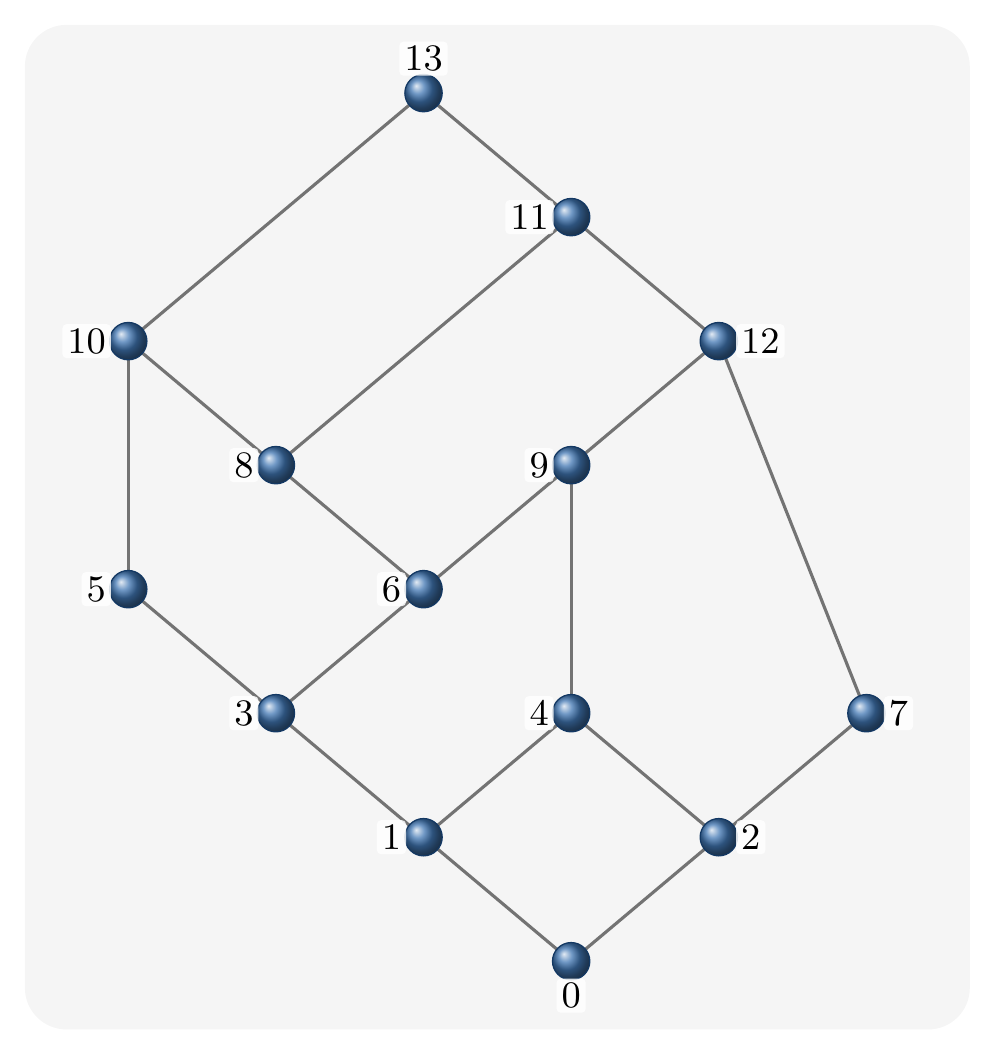
\includegraphics[width=0.46\textwidth]{figures/k14.png}
\caption{The semidistributive lattice $K$.}\label{fig:K}
\end{figure}

\begin{table}[t]
\centering
\small
\begin{tabular}{cccc@{\qquad}cccc}
\toprule
$j$ & $j_*$ & $\up j_*\setminus\up j$ & $\kappa(j)$ & $m$ & $m^*$ & $\dn m^*\setminus\dn m$ & $\kappa^d(m)$\\
\midrule
$1$ & $0$ & $\{0,2,7\}$ & $7$ & $4$ & $9$ & $\{3,6,9\}$ & $3$\\
$2$ & $0$ & $\{0,1,3,5,6,8,10\}$ & $10$ & $5$ & $10$ & $\{6,8,10\}$ & $6$\\
$3$ & $1$ & $\{1,4\}$ & $4$ & $7$ & $12$ & $\{1,3,4,6,9,12\}$ & $1$\\
$5$ & $3$ & $\{3,6,8,9,11,12\}$ & $11$ & $9$ & $12$ & $\{7,12\}$ & $7$\\
$6$ & $3$ & $\{3,5\}$ & $5$ & $10$ & $13$ & $\{2,4,7,9,11,12,13\}$ & $2$\\
$7$ & $2$ & $\{2,4,9\}$ & $9$ & $11$ & $13$ & $\{5,10,13\}$ & $5$\\
$8$ & $6$ & $\{6,9,12\}$ & $12$ & $12$ & $11$ & $\{8,11\}$ & $8$\\
\bottomrule
\end{tabular}
\medskip
\caption{The sets of Lemma~\ref{lem:kappa} for $K$, with their greatest and least elements.}\label{tab:kappa}
\end{table}

\begin{proposition}\label{prop:K}
$K$ is semidistributive.
\end{proposition}

\begin{proof}
Table~\ref{tab:kappa} lists, for each join-irreducible $j$, the set $\up j_*\setminus\up j$ of elements above $j_*$ and not above $j$, and for each meet-irreducible $m$ the set $\dn m^*\setminus\dn m$. Each of the fourteen sets has a greatest, respectively least, element, shown in the table; for instance $\up3\setminus\up5=\{3,6,8,9,11,12\}$ has greatest element $11$, since $3\le6\le8\le11$ and $9\le12\le11$. Lemma~\ref{lem:kappa} gives both semidistributive laws.
\end{proof}

\begin{remark}\label{rem:D}
$K$ is not lower bounded, so it is not bounded. Recall that for join-irreducible $p\ne q$ one writes $p\mathrel{D}q$ if $p\le q\vee x$ and $p\not\le q_*\vee x$ for some $x$, and that a finite lattice is lower bounded exactly when this relation has no cycle (see~\cite[Chapter~II]{FJN} and~\cite{Da}). In $K$,
\begin{align*}
6&\le 7\vee1=12, & 7&\le 8\vee2=11, & 8&\le 6\vee5=10,\\
6&\not\le 2\vee1=4, & 7&\not\le 6\vee2=9, & 8&\not\le 3\vee5=5,
\end{align*}
so $6\mathrel{D}7\mathrel{D}8\mathrel{D}6$. By the theorem of Adams, Freese, Nation and Schmid this, or the dual phenomenon, is unavoidable in any counterexample.
\end{remark}

\section{The lattice \texorpdfstring{$L$}{L} and its diagonal}

Define $\varphi\colon K\to K$ and $\psi\colon K\to K$ by Table~\ref{tab:phi}.

\begin{table}[t]
\centering
\small
\setlength{\tabcolsep}{4.5pt}
\begin{tabular}{c*{14}{c}}
\toprule
$x$ & $0$ & $1$ & $2$ & $3$ & $4$ & $5$ & $6$ & $7$ & $8$ & $9$ & $10$ & $11$ & $12$ & $13$\\
\midrule
$\varphi(x)$ & $0$ & $6$ & $7$ & $8$ & $12$ & $10$ & $8$ & $7$ & $8$ & $11$ & $10$ & $11$ & $11$ & $13$\\
$\psi(x)$ & $0$ & $1$ & $2$ & $1$ & $4$ & $5$ & $1$ & $2$ & $3$ & $4$ & $5$ & $9$ & $4$ & $13$\\
\midrule
$[x,\varphi(x)]$ & $0$ & $1,3,6$ & $2,7$ & $3,6,8$ & $4,9,12$ & $5,10$ & $6,8$ & $7$ & $8$ & $9,12,11$ & $10$ & $11$ & $12,11$ & $13$\\
\bottomrule
\end{tabular}
\medskip
\caption{The maps $\varphi$ and $\psi$, and the intervals $[x,\varphi(x)]$ of $K$.}\label{tab:phi}
\end{table}

\begin{lemma}\label{lem:L}
The set $L=L_\varphi=\{(x,y)\in K\times K: x\le y\le\varphi(x)\}$ is a sublattice of $K\times K$ with $26$ elements. It consists of the diagonal $D=\{(x,x):x\in K\}$ and the twelve pairs
\[
(1,3),\ (1,6),\ (2,7),\ (3,6),\ (3,8),\ (4,9),\ (4,12),\ (5,10),\ (6,8),\ (9,11),\ (9,12),\ (12,11).
\]
In particular $L$ is semidistributive.
\end{lemma}

\begin{proof}
Clearly $x\le\varphi(x)$ for every $x$. For each $y$ the set $\{x: y\le\varphi(x)\}$ is the filter $\up\psi(y)$. For example, the values of $\varphi$ above $6$ are taken exactly on $K\setminus\{0,2,7\}=\up1$, and $\psi(6)=1$; the other thirteen cases are checked in the same way from Figure~\ref{fig:K}. Lemma~\ref{lem:Lphi} shows that $L$ is a sublattice. Its elements are the pairs $(x,y)$ with $y$ in the interval $[x,\varphi(x)]$ listed in the last row of Table~\ref{tab:phi}, which gives $26$ pairs, fourteen of them on the diagonal. Finally $K\times K$ is semidistributive by Proposition~\ref{prop:K}, and so is its sublattice $L$.
\end{proof}

Write $C=L\setminus D$ for the twelve pairs off the diagonal and $\bar d=(d,d)$ for the diagonal elements; Figure~\ref{fig:L} shows $L$. The following computation, performed coordinatewise in $K$, is the heart of the example:
\begin{equation}\label{eq:cycle}
\begin{aligned}
(1,3)\vee\bar2&=(4,9), & (4,9)\wedge\overline{10}&=(1,6), & (1,6)\vee\bar3&=(3,6),\\
(3,6)\vee\bar5&=(5,10), & (5,10)\wedge\overline{11}&=(3,8), & (3,8)\vee\bar7&=(12,11),\\
(12,11)\wedge\bar8&=(6,8), & (6,8)\vee\bar2&=(9,11), & (9,11)\wedge\overline{12}&=(9,12),\\
(9,12)\wedge\bar7&=(2,7), & (2,7)\vee\bar1&=(4,12), & (4,12)\wedge\bar3&=(1,3).
\end{aligned}
\end{equation}
Starting from any pair of $C$ and joining or meeting with diagonal elements, one runs through all of $C$ and returns.\footnote{In the first coordinate, for example, $1\vee2=4$, $4\wedge10=1$, $1\vee3=3$, $3\vee5=5$, $5\wedge11=3$, $3\vee7=12$; in the second, $3\vee2=9$, $9\wedge10=6$, $6\vee3=6$, $6\vee5=10$, $10\wedge11=8$, $8\vee7=11$. The remaining six steps are read off Figure~\ref{fig:K} in the same way.}

\begin{figure}[t]
\centering
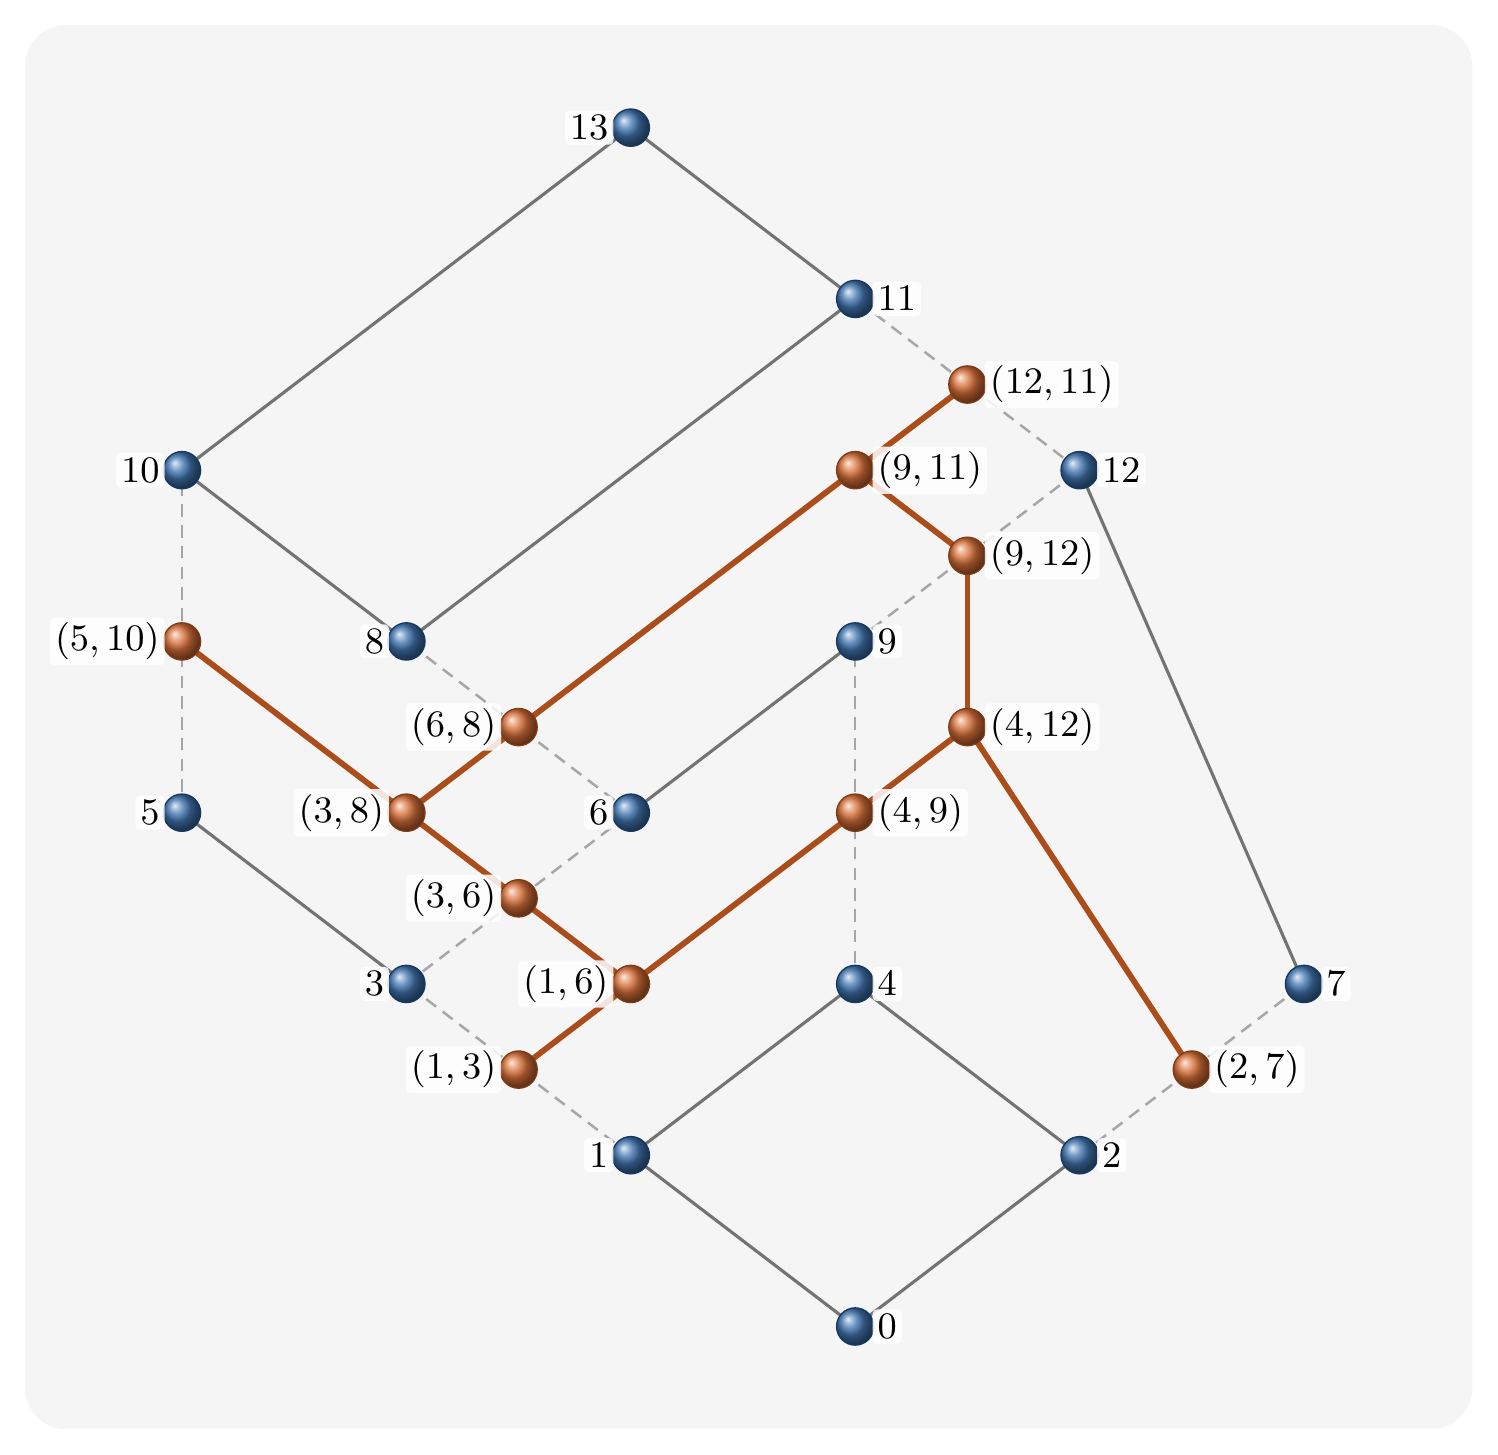
\includegraphics[width=0.66\textwidth]{figures/l26.png}
\caption{The lattice $L$. The diagonal $D\cong K$ is shown in blue and labelled by $d$ for $(d,d)$; the complement $C$ is shown in orange. Dashed lines are covering pairs between $D$ and $C$.}\label{fig:L}
\end{figure}

\begin{proposition}\label{prop:max}
$D$ is a maximal proper sublattice of $L$.
\end{proposition}

\begin{proof}
$D$ is a sublattice, and it is proper because $C\ne\varnothing$. Let $S$ be a sublattice of $L$ with $D\subsetneq S$, and pick $c\in S\setminus D$. Each step of~\eqref{eq:cycle} joins or meets an element of $C$ with an element of $D\subseteq S$, and the twelve steps form a single cycle through all of $C$. Following the cycle from $c$ shows $C\subseteq S$, so $S=D\cup C=L$.
\end{proof}

\begin{theorem}\label{thm:main}
$L$ is a semidistributive lattice with $26$ elements, $D$ is a maximal proper sublattice of $L$, and the complement $C=L\setminus D$ has the two minimal elements $(1,3)$ and $(2,7)$ and the two maximal elements $(5,10)$ and $(12,11)$. Consequently $C$ is not an interval and is not order convex. In particular the question of Adams, Freese, Nation and Schmid has a negative answer, and the conjecture of Adaricheva, Mata, Silberger and Zamojska-Dzienio is false.
\end{theorem}

\begin{proof}
The first two assertions are Lemma~\ref{lem:L} and Proposition~\ref{prop:max}. The elements of $L$ below $(1,3)$ are the pairs $(x,y)$ with $x\le1$ and $y\le3$, namely $(0,0)$, $(1,1)$ and $(1,3)$, and those below $(2,7)$ are $(0,0)$, $(2,2)$ and $(2,7)$. So both are minimal in $C$, and they are incomparable. Dually, the elements of $L$ above $(5,10)$ are $(5,10)$, $(10,10)$ and $(13,13)$, and those above $(12,11)$ are $(12,11)$, $(11,11)$ and $(13,13)$, so both are maximal in $C$.

If $C$ were an interval $[u,w]$, then $u\le(1,3)\wedge(2,7)=(0,0)\le(1,3)\le w$, so the diagonal element $(0,0)$ would lie in $C$. Hence $C$ is not an interval. It is not order convex either, since $(1,3)<(3,3)<(3,6)$ with $(1,3),(3,6)\in C$ and $(3,3)\in D$.

By~\cite[Theorem~7]{AFNS} the complement of a maximal sublattice $M$ of a bounded lattice is an interval $[v,u]$ with $u\in\operatorname{CM}(v)$ and $v\in\operatorname{CJ}(u)$; the asked extension to semidistributive lattices would force $C$ to be such an interval, and the conjecture of~\cite{AMSZ} would force $C$ to be an interval. Neither holds.
\end{proof}

\section{Remarks}

\begin{remark}
$L$ is the sublattice of $K\times K$ generated by $D$ and the single pair $(1,3)$: the cycle~\eqref{eq:cycle} produces every pair of $C$ from $(1,3)$ and the diagonal. Exchanging the two coordinates gives an isomorphic example generated by $D$ and $(3,1)$. The example was found by a computer search over sublattices of $A\times A/\theta$ generated by the graph of the quotient map and a few further pairs, for small semidistributive lattices $A$ that are not bounded and congruences $\theta$ of $A$ (here $\theta$ is trivial and the graph is the diagonal); among the $46$ sublattices of $K\times K$ generated by the diagonal and one further pair, these two are the smallest, and both give counterexamples. No step of the proof above depends on that search.
\end{remark}

\begin{remark}
The diagonal is not a maximal sublattice of $K\times K$ itself, since it lies strictly inside $L$. Passing to $L$, which keeps only the pairs $(x,y)$ with $y$ in the interval $[x,\varphi(x)]$, removes every sublattice strictly between the diagonal and the whole lattice. The lattice $K$ is self-dual (the map $0,1,2,3,4,5,6,7,8,9,10,11,12,13\mapsto13,11,10,12,8,7,9,5,4,6,2,1,3,0$ reverses the order), and by~\cite[Theorem~E and its proof]{Bh} it is, up to isomorphism, the only semidistributive lattice with at most fourteen elements that is not bounded.
\end{remark}

By~\cite[Theorem~E]{Bh}, every semidistributive lattice with at most fourteen elements satisfies the conjecture, so the smallest counterexample has between $15$ and $26$ elements.

\begin{question}
What is the least size of a finite semidistributive lattice with a maximal sublattice whose complement is not an interval?
\end{question}

\subsection*{Formal verification}
The statement of Theorem~\ref{thm:main} is formalized in Lean~4~\cite{MU} with Mathlib~\cite{Mathlib}: the lattices $K$ and $L$ are given by their operation tables, the embedding of $L$ into $K\times K$ is checked to be an injective lattice homomorphism, both semidistributive laws are checked by the kernel, and maximality of $D$ is proved by the twelve steps of~\eqref{eq:cycle}. The main theorem depends only on the standard axioms of Lean. The development and the search programs are archived in~\cite{Ar}.

\subsection*{Use of generative AI}
The author used Claude (Anthropic) to search for the example, to check it by computer and in Lean, and to draft the text; the author verified every step and is responsible for the content.

\begin{thebibliography}{99}

\bibitem{AFNS}
M.~E.~Adams, R.~Freese, J.~B.~Nation and J.~Schmid, \emph{Maximal sublattices and Frattini sublattices of bounded lattices}, J. Austral. Math. Soc. Ser.~A \textbf{63} (1997), 110--127. \doi{10.1017/S1446788700000355}

\bibitem{AMSZ}
K.~Adaricheva, A.~Mata, S.~Silberger and A.~Zamojska-Dzienio, \emph{Conjecture on maximal sublattices of finite semidistributive lattices and beyond}, Discrete Math. Theor. Comput. Sci. \textbf{28}:2 (2026). \doi{10.46298/dmtcs.16374}

\bibitem{Ar}
D.~Bhattacharjee, \emph{Maximal sublattices of finite semidistributive lattices: paper, Lean~4 development and search programs}, 2026. \url{https://github.com/creelie/Conjecture-001}

\bibitem{Bh}
D.~Bhattacharjee, \emph{Maximal sublattices of convex geometries: four counterexamples}, Zenodo, 2026. \doi{10.5281/zenodo.23343145}

\bibitem{CKT}
C.~C.~Chen, K.~M.~Koh and S.~K.~Tan, \emph{Frattini sublattices of distributive lattices}, Algebra Universalis \textbf{3} (1973), 294--303. \doi{10.1007/BF02945131}

\bibitem{Da}
A.~Day, \emph{Characterizations of finite lattices that are bounded-homomorphic images or sublattices of free lattices}, Canad. J. Math. \textbf{31} (1979), 69--78. \doi{10.4153/CJM-1979-008-x}

\bibitem{FJN}
R.~Freese, J.~Je\v{z}ek and J.~B.~Nation, \emph{Free Lattices}, Mathematical Surveys and Monographs \textbf{42}, American Mathematical Society, Providence, RI, 1995. \doi{10.1090/surv/042}

\bibitem{Mathlib}
The mathlib Community, \emph{The Lean mathematical library}, in: Proceedings of the 9th ACM SIGPLAN International Conference on Certified Programs and Proofs (CPP 2020), ACM, New York, 2020, 367--381. \doi{10.1145/3372885.3373824}

\bibitem{MU}
L.~de~Moura and S.~Ullrich, \emph{The Lean~4 theorem prover and programming language}, in: Automated Deduction -- CADE~28, Lecture Notes in Comput. Sci. \textbf{12699}, Springer, Cham, 2021, 625--635. \doi{10.1007/978-3-030-79876-5_37}

\bibitem{Ri}
I.~Rival, \emph{Maximal sublattices of finite distributive lattices}, Proc. Amer. Math. Soc. \textbf{37} (1973), 417--420. \doi{10.1090/S0002-9939-1973-0311527-9}

\end{thebibliography}

\end{document}
